\section*{Kapitel 5 - Metrische Einflußgrößen}

\begin{multicols*}{3}

\tikzstyle{mybox} = [draw=black, fill=white, very thick,
    rectangle, rounded corners, inner sep=10pt, inner ysep=10pt]
\tikzstyle{fancytitle} =[fill=black, text=white, font=\bfseries]



%------------ Interaktion metrischer Variablen ---------------
\begin{tikzpicture}
    \node [mybox] (box){%
        \begin{minipage}{0.3\textwidth}
        Seien $X_1, X_2$ zwei metrische Variablen mit den Ausprägungen $x_{1i}, x_{2i}$ für $i = 1, \dots, n$.
        Die Modellgleichung für das Modell mit Interaktion 
        lautet:
        \begin{align*}
            Y_i &= \beta_0 + \beta_1 x_{1i} + \beta_2 x_{2i} + \beta_3 x_{1i} x_{2i} + \epsilon_i\\
                &= \beta_0 + \beta_2 x_{2i} + (\beta_1 + \beta_3 x_{2i})x_{1i}  + \epsilon_i\\
                &= \beta_0 + \beta_1 x_{1i} + (\beta_2 + \beta_3 x_{1i})x_{2i}  + \epsilon_i
        \end{align*}

        Interpreation der Modellparameter:\\
        Die Parameter $\gb{1}, \gb{2}$ geben die Steigung bei $x_1 = x_2 = 0$ an. I.d.R.
        nicht sinnvoll interpretierbar.
        

    \end{minipage}
    };
%------------ Interaktion metrischer Variablen Header ---------------------
\node[fill = black, text=white, font=\bfseries, right=10pt] at (box.north west) 
{Interaktion metrischer Variablen};
\end{tikzpicture}

%------------ Modelle mit metrischen Variablen ---------------
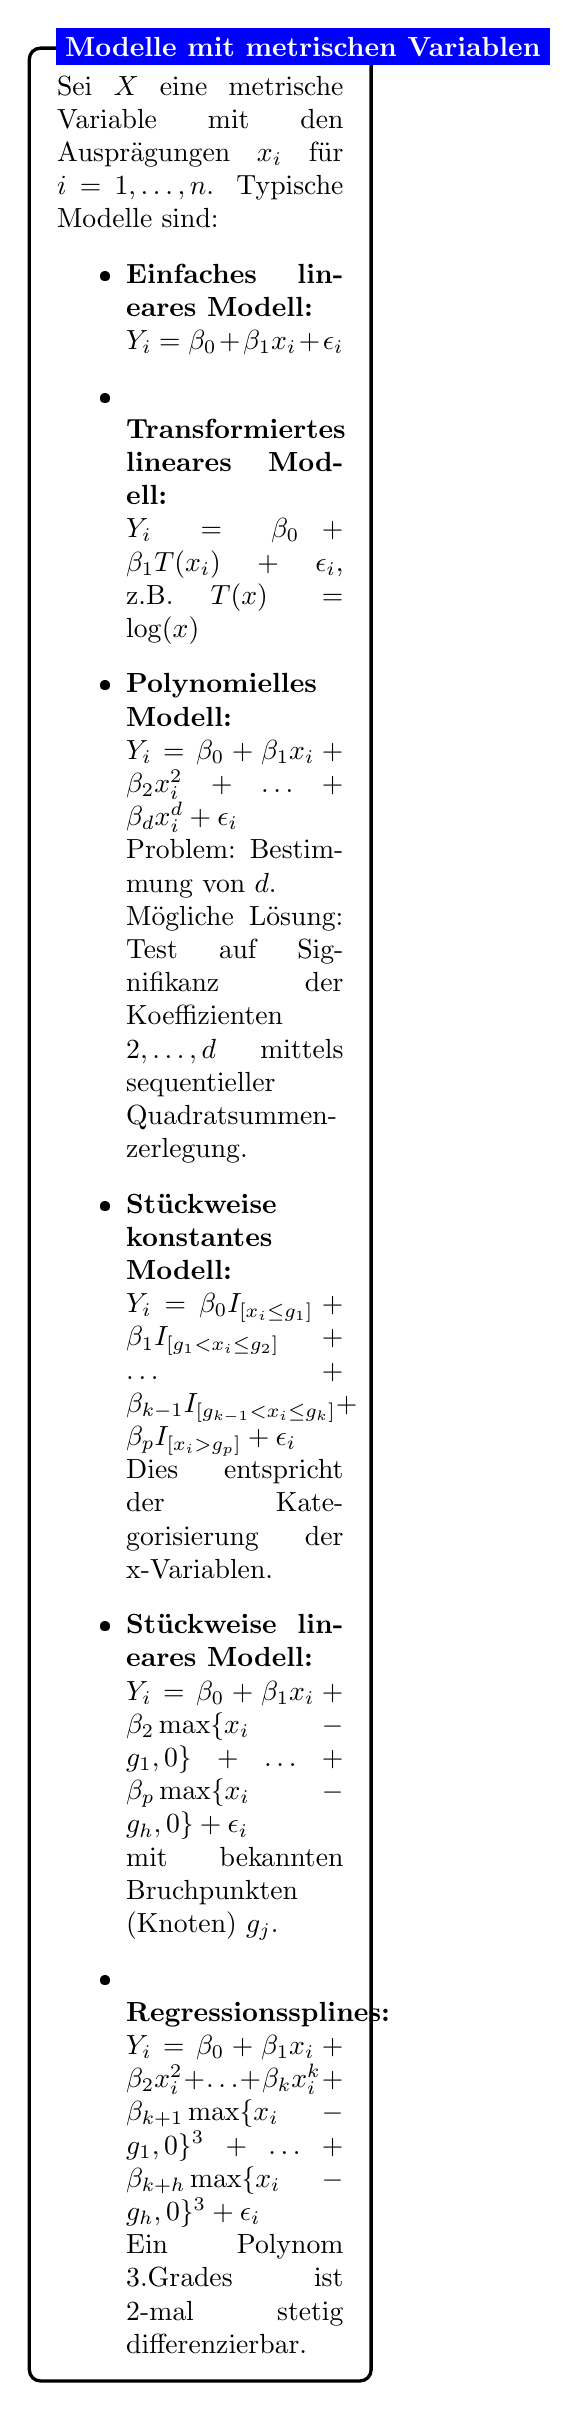
\begin{tikzpicture}
    \node [mybox] (box){%
        \begin{minipage}{0.3\textwidth}
        Sei $X$ eine metrische Variable mit den Ausprägungen $x_{i}$ für $i = 1, \dots, n$. Typische Modelle sind:
        \begin{itemize}
            \item \textbf{Einfaches lineares Modell:} \\
            $Y_i = \beta_0 + \beta_1 x_{i} + \epsilon_i$
            \item \textbf{Transformiertes lineares Modell:} \\
            $Y_i = \beta_0 + \beta_1 T(x_{i}) + \epsilon_i$, \quad z.B. $T(x) = \log(x)$
            \item \textbf{Polynomielles Modell:} \\
            $Y_i = \beta_0 + \beta_1 x_{i} + \beta_2 x_{i}^2 + \dots + \beta_d x_{i}^d + \epsilon_i$\\
            Problem: Bestimmung von $d$.\\
            Mögliche Lösung: Test auf Signifikanz der Koeffizienten $\gb{2},
            \dots, \gb{d}$ mittels sequentieller Quadratsummenzerlegung.
            \item \textbf{Stückweise konstantes Modell:} \\
            $Y_i = \beta_0 I_{[x_{i} \leq g_1]} + \beta_1 I_{[g_1 < x_{i} \leq
            g_2]} + \dots + \beta_{k-1} I_{[g_{k-1} < x_{i} \leq g_k]} +
            \beta_{p} I_{[x_{i} > g_p]} + \epsilon_i$\\
            Dies entspricht der Kategorisierung der x-Variablen.
            \item \textbf{Stückweise lineares Modell:} \\
            $Y_i = \beta_0 + \beta_1 x_{i} + \beta_2 \max\{x_i-g_1, 0\} + \dots
            + \beta_{p} \max\{x_i-g_{h}, 0\} + \epsilon_i$\\
            mit bekannten Bruchpunkten (Knoten) $g_j$.
            \item \textbf{Regressionssplines:} \\
            $Y_i = \beta_0 + \beta_1 x_{i} + \beta_2 x_i^2 + \dots + \beta_{k}
            x_i^{k} + \beta_{k + 1} \max\{x_i - g_1, 0\}^3 + \dots + \beta_{k +
            h} \max\{x_i - g_h, 0\}^3 + \epsilon_i$\\
            Ein Polynom 3.Grades ist 2-mal stetig differenzierbar.
        \end{itemize}
        

    \end{minipage}
    };
%------------ Modelle mit metrischen Variablen Header ---------------------
\node[fill = blue, text=white, font=\bfseries, right=10pt] at (box.north west) 
{Modelle mit metrischen Variablen};
\end{tikzpicture}


%------------ Allgemeiner Ansatz mit Basisfunktionen ---------------
\begin{tikzpicture}
    \node [mybox] (box){%
        \begin{minipage}{0.3\textwidth}
        Sei $X$ eine metrische Variable mit den Ausprägungen $x_{i}$ für $i = 1, \dots, n$.\\
        Allgemeiner Ansatz für Modelle mit Basisfunktionen:\\
        Seien $B_1, B_2, \dots, B_k$ Basisfunktionen. Dann ist die allgemeine Modellgleichung:
        \begin{align*}
            Y_i &= \beta_0 + \beta_1 B_1(x_{i}) + \beta_2 B_2(x_{i}) + \dots + \beta_k B_k(x_{i}) + \epsilon_i
        \end{align*}

    \end{minipage}
    };
%------------ Allgemeiner Ansatz mit Basisfunktionen Header ---------------------
\node[fill = purple, text=white, font=\bfseries, right=10pt] at (box.north west) 
{Allgemeiner Ansatz mit Basisfunktionen};
\end{tikzpicture}


\end{multicols*}